% =============================================================================
% PCDS 2026 camera-ready (5 pages incl. references). IEEE conference format, US
% Letter, matching the official PCDS "Proceeding-Template.doc" (IEEE template).
% =============================================================================
\documentclass[conference]{IEEEtran}
\IEEEoverridecommandlockouts
\usepackage{cite}
\usepackage{amsmath,amssymb,amsfonts}
\usepackage{graphicx}
\usepackage{booktabs}
\usepackage{textcomp}
\usepackage{xcolor}
\usepackage{url}
\urlstyle{same}
\renewcommand{\IEEEkeywordsname}{Keywords}
\newcommand{\authoremail}[1]{{\small #1}}
\newcommand{\tabnote}[1]{\par\vspace{2pt}\parbox{\columnwidth}{\scriptsize #1}}

\makeatletter
\newcommand{\linebreakand}{\end{@IEEEauthorhalign}\hfill\mbox{}\par\mbox{}\hfill\begin{@IEEEauthorhalign}}
\makeatother

\begin{document}

\title{Growing Prefixes Meet Finite Caches: When Does Eviction-Aware Routing Pay Off for Agentic LLM Serving?}

\author{
\IEEEauthorblockN{Akhil Varun Varma Kalidindi}
\IEEEauthorblockA{\textit{Dept. of Computer Science} \\
\textit{and Engineering} \\
\textit{\'Ecole Centrale School of Engineering}\\
\textit{Mahindra University}\\
Telangana, India-500043 \\
\authoremail{se24uari028@mahindrauniversity.edu.in}}
\and
\IEEEauthorblockN{Manda Siddharth}
\IEEEauthorblockA{\textit{Dept. of Computer Science} \\
\textit{and Engineering} \\
\textit{\'Ecole Centrale School of Engineering}\\
\textit{Mahindra University}\\
Telangana, India-500043 \\
\authoremail{se24uari039@mahindrauniversity.edu.in}}
\and
\IEEEauthorblockN{Rishi Kamishetty}
\IEEEauthorblockA{\textit{Dept. of Computer Science} \\
\textit{and Engineering} \\
\textit{\'Ecole Centrale School of Engineering}\\
\textit{Mahindra University}\\
Telangana, India-500043 \\
\authoremail{se24uari025@mahindrauniversity.edu.in}}
\linebreakand
\IEEEauthorblockN{Bilakanti Mukesh Reddy}
\IEEEauthorblockA{\textit{Dept. of Computer Science} \\
\textit{and Engineering} \\
\textit{\'Ecole Centrale School of Engineering}\\
\textit{Mahindra University}\\
Telangana, India-500043 \\
\authoremail{se24uari026@mahindrauniversity.edu.in}}
\and
\IEEEauthorblockN{Lakshmi Pavan Rangisetti}
\IEEEauthorblockA{\textit{Dept. of Computer Science} \\
\textit{and Engineering} \\
\textit{\'Ecole Centrale School of Engineering}\\
\textit{Mahindra University}\\
Telangana, India-500043 \\
\authoremail{se24uari015@mahindrauniversity.edu.in}}
\and
\IEEEauthorblockN{Veeraiah Talagondapati*}
\IEEEauthorblockA{\textit{Dept. of Computer Science} \\
\textit{and Engineering} \\
\textit{\'Ecole Centrale School of Engineering}\\
\textit{Mahindra University}\\
Telangana, India-500043 \\
\authoremail{veeraiah.talagondapati@}\\
\authoremail{mahindrauniversity.edu.in}}
}

\maketitle

\begin{abstract}
Cache-aware routers send LLM requests that share a prompt prefix to the replica that already caches it. For agentic workloads, whose prompts grow with every tool call, session-centric routing with a guard against evicted sessions beats both load balancing and pure cache affinity; we ask when that guard pays off. The deciding variable is tool-call latency: it sets the reusable working set that competes for per-replica KV memory. Using TTFT measurements in vLLM and a simulator calibrated on them, we compare eight routing policies over median tool latencies of 50~ms--60~s, with KV capacity set relative to the working set or fixed in tokens. On agentic traffic, cache-aware routing lowers p95 TTFT from 155 to 60~ms ($-$61\%) at unchanged throughput. An eviction-aware, TTFT-estimating router first leads the best eviction-oblivious locality policy by $\ge$5\% (paired 95\% CI excluding zero) at 5~s when capacity does not exceed the working set (agentic 7.5$\pm$3.9\%, 6~ms; synthetic 17$\pm$4\%, 38~ms), at 0.5--1~s when headroom is scarce, and at 10~s even with ample memory; its agentic lead grows to about 20\% (54--56~ms) at 30--60~s. Its misses are not cheaper: it cuts the tail share spent waiting behind other requests from 23--51\% to 4--7\%, and ablations show that queue-aware placement is the necessary ingredient. Multi-replica results are simulated.
\end{abstract}

\begin{IEEEkeywords}
LLM serving, KV cache, prefix caching, request routing, load balancing, agentic workloads, performance modelling
\end{IEEEkeywords}

% =============================================================================
\section{Introduction}
\label{sec:intro}

A production LLM service runs many replicas behind a router. Engines such as vLLM~\cite{r1} and SGLang~\cite{r2} skip the prefill of cached prompt prefixes, and routers such as Preble~\cite{r3}, the SGLang router~\cite{r4}, NVIDIA Dynamo~\cite{r5}, llm-d~\cite{r6} and the vLLM production stack~\cite{r7} trade this locality against load balance, mostly tuned on chat traffic with stable shared prefixes. In agentic workloads each tool result is appended to the context, so a session's reusable prefix grows strictly and the \emph{reusable working set} scales with the number of sessions waiting on tools. SMetric~\cite{r8} finds over 80\% of agentic prompt tokens reusable and guards session stickiness against eviction; CacheRoute~\cite{r9} measures when prefix affinity should give way to load balancing. What remains open is \emph{when the eviction guard matters}, which depends on tool latency and on the KV memory left for idle sessions.

Proposing no new algorithm (our eviction-aware router is an idealised form of SMetric's scheduler), we contribute by measurement and trace-driven simulation: (1) \emph{tool-call latency as a first-class parameter}, swept from 50~ms to 60~s with normalised and fixed KV capacity to locate the crossover from which eviction-aware routing beats eviction-oblivious locality; (2) \emph{the mechanism}, isolated by a miss-cost decomposition and ablations; (3) \emph{a measured cost model with bracketed simulator bias}, against which every effect is reported in absolute and relative terms, and an output-correctness check of prefix caching; (4) policy rankings, throughput and routing guidance.

% =============================================================================
\section{Background and Related Work}
\label{sec:related}

vLLM keeps the keys and values (KV) of processed tokens in fixed-size blocks~\cite{r1}; automatic prefix caching lets a request skip the prefill of its longest run of resident leading blocks, and unreferenced blocks are evicted LRU~\cite{r10}. Routers use consistent hashing on a prefix~\cite{r11}, longest-prefix matching with a load fallback~\cite{r4}, or session affinity~\cite{r7}; load-only baselines ignore the cache. Preble~\cite{r3} co-schedules prefix sharing and load; multi-turn and agentic systems retain or schedule KV state on one engine~\cite{r15,r16,r19,r20}. \textbf{SMetric}~\cite{r8} places first-turn requests by estimated queued plus own prefill and keeps follow-ups on the highest-hit replica unless a \texttt{session\_cached} check detects eviction; it varies a global KV tier on 32 H20 GPUs, but not per-instance capacity or tool latency. \textbf{CacheRoute}~\cite{r9} plans affinity and load jointly but models neither tool gaps nor evicted sessions nor per-replica capacity. Anyscale~\cite{r21} compares session, prefix and load-aware routing on agent traces; MISA-T~\cite{r22} reports cache-aware routing failing under KV contention.

% =============================================================================
\section{Measurement Study (RQ1)}
\label{sec:measure}

\textbf{Setup.} vLLM 0.8.5.post1 (V1 engine, 8192-token chunked prefill) serves Qwen2.5-7B-Instruct-AWQ~\cite{r23} on a \emph{4g.20gb MIG slice} of an A100-SXM4-40GB (KV capacity 194,368 tokens). A prompt of length $L$ with hit fraction $h$ is a warmed shared prefix of $hL$ tokens plus a random suffix. We sweep $h\in\{0,.25,.5,.75,.9,1\}$, $L\in\{1,4,8,16\}$k and $c\in\{1,4,16,32\}$ closed-loop clients, with caching on and off and 64 greedy output tokens, plus a small-cache configuration (32k tokens).

\begin{figure}[t]
\centering
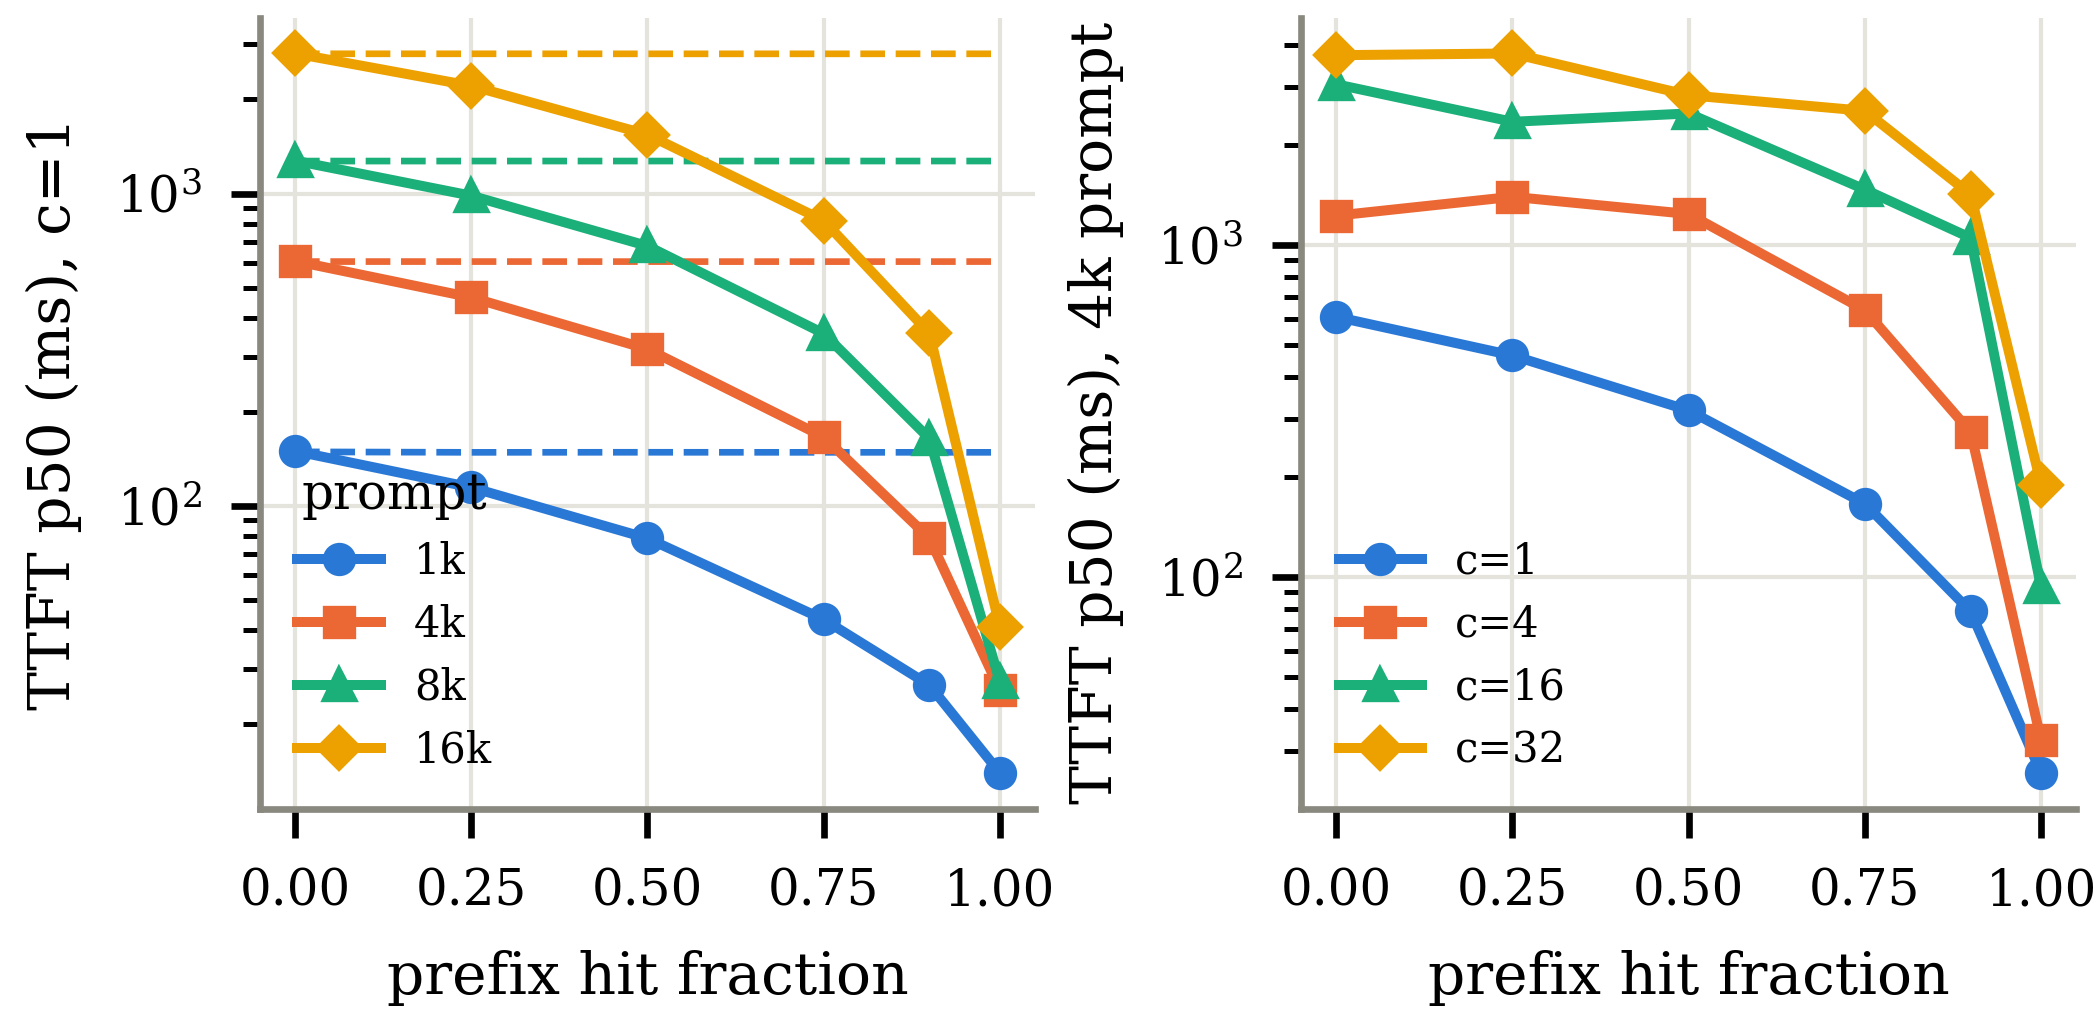
\includegraphics[width=0.78\columnwidth]{figs/fig1_ttft.png}
\caption{Measured median TTFT (A100 4g.20gb MIG, vLLM 0.8.5, Qwen2.5-7B-AWQ). Left: isolated requests by prompt length; solid = caching on, dashed = off. Right: 4k-token prompts at increasing concurrency.}
\label{fig:ttft}
\end{figure}

\textbf{Results.} TTFT falls almost linearly in the number of \emph{uncached} tokens (Fig.~\ref{fig:ttft}): for 8k-token prompts from 1274~ms at $h=0$ to 164~ms at $h=0.9$ (7.8$\times$), at 16k from 2808 to 357~ms; with nothing to reuse, caching changes TTFT by +0\%. At $c=16$ and 16k tokens queueing dominates (17861~ms without reuse, 3012~ms at $h=0.9$). With the 32k-token cache at $c=16$ and no reuse, KV utilisation peaks at 89\%, the engine performs 8.9$\times$ the prefix-cache lookups a single pass needs and median TTFT rises 2.3$\times$ (4.9$\times$ at $c=32$), while at $h=0.9$ it is unchanged: memory pressure makes each miss more expensive. \textbf{Cost model.} Non-negative least squares on isolated-request TTFTs and steady-state ITLs fits the per-iteration cost $T_{\mathrm{iter}}=a+bP+cD+d_pA_p+d_dA_d$ ($P$: prefill tokens; $D$: decoding sequences; $A_p$, $A_d$: prefill and decode attention work) with $a=9.94$~ms, $b=135.1$~$\mu$s/token, $c=114.3$~$\mu$s/seq, $d_p=4.56$~$\mu$s, $d_d=40.8$~$\mu$s ($R^2=0.972$; TTFT MAPE 6.2\%). \textbf{Correctness.} A companion deployment had disabled prefix caching after observing output divergence, so we compare greedy completions token by token in a 300-session replay (1047 completions) run twice per configuration. Two identical caching-off runs agree on only 82.3\%: batch composition changes the floating-point reduction order. Against this run-to-run control, caching on vs.\ off agrees on 83.1\%; paired on the same completions the difference is not significant (60 vs.\ 52 discordant, exact McNemar $p=0.51$; session-bootstrap 95\% CI $-1.2$ to $+2.7$ points), so prefix caching adds no detectable divergence. With caching on, 2 of 8 sequential probes change their continuation between a cold and a warm cache (after $\sim$30 tokens) while repeated caching-off runs are identical: the cached-prefix path is numerically, not semantically, different.

% =============================================================================
\section{Simulator and Calibration}
\label{sec:sim}

\textbf{Replica model.} Each replica is an iteration-level model of a vLLM V1 engine (FCFS admission when blocks fit, reusing the longest resident prefix; one token per decoding sequence and the remaining budget for prefill chunks per iteration; finished blocks cached until LRU-evicted), with blocks following each session's token lineage. \textbf{Validation and bias.} Over 205 replayed benchmark settings the median TTFT residual is $-$1.9\% (Spearman $\rho=0.99$) and flat across hit fractions ($-$1.8\% at $h=0$, $-$2.6\% at $h=0.9$), so the miss penalty is reproduced to within 2\%. The one systematic error, at full hits ($-$73\% at $h=1$), arises because the model treats cached tokens as free, whereas the engine charges about 1.47~$\mu$s each; adding that term moves the residual to +0.2\%, so the two cost models bracket the engine, and we re-simulate the key cells with it. On a 300-session multi-turn replay the error is $-$29\%/$-$15\% (median/p95), and $-$21\%/$-$23\% with the term. \textbf{Workloads.} \emph{Chat}: the Azure LLM inference trace~\cite{r24,r25} with 16 synthesised system-prompt templates (Zipf(1.1), median 600 tokens). \emph{Agentic}: a numeric descriptor of a companion tool-calling agent (19,505 sessions, 79,703 turns), with prompt lengths reconstructed via the append-only structure. \emph{Synthetic agentic}: sessions drawn from distributions fitted to that trace. Arrivals are Poisson at 70\% nominal utilisation; turns within a session are closed-loop. \textbf{Tool latency.} Measured tool latencies range from tens of ms (local tools; median 166~ms in Copilot sessions) to 0.7--2.7~s on average for web and shell tools~\cite{r16,r19,r20,r26,r27,r28,r29}, and builds, tests and sub-agents take longer. We rescale each session's gaps by a common factor, keeping their shape, to median tool latencies $\tau$ of 50, 200, 500~ms and 1, 2, 5, 10, 15, 30, 60~s.

\textbf{KV capacity and $\kappa$.} Per-replica capacity is
\begin{equation}
C=H+\kappa\,\frac{W(\tau)}{N},\qquad H=2F+M_{\max},
\label{eq:cap}
\end{equation}
with $F$ the nominal in-flight footprint per replica, $M_{\max}$ the largest request, $N=4$ replicas, and $W(\tau)$ the \emph{reusable working set}: the time-averaged footprint of shared templates plus contexts of sessions between turns. By Little's law its idle part is about $\lambda_t\bar\tau\bar S$ (tool-call rate, mean tool latency, mean context), so $W$ grows linearly with $\tau$. $\kappa<1$ means the cluster cannot keep every idle context, $\kappa=1$ that it just can, $\kappa>1$ that it has room to spare; we use $\kappa\in\{0.25,0.5,1,2\}$ and nominal or halved $H$. Because $C$ scales with $W(\tau)$, raising $\tau$ at fixed $\kappa$ raises the absolute capacity but shrinks the headroom's share of it; the room for idle sessions relative to their demand,
\begin{equation}
\rho(\tau)=\frac{C}{W(\tau)/N}=\kappa+\frac{N H}{W(\tau)},
\label{eq:rho}
\end{equation}
falls from far above $\kappa$ towards $\kappa$ as $\tau$ grows. A deployment instead fixes $C$, so $\rho$ falls as $1/W(\tau)$; we therefore also sweep $\tau$ at fixed absolute $C$ (the $\kappa=1$, $\tau=1$~s capacity: 1020 blocks agentic, 740 synthetic).

% =============================================================================
\section{Routing Policies}
\label{sec:policies}

\emph{Round-robin}, \emph{random} and \emph{least-loaded} ignore the cache; \emph{session affinity} hashes the session id; \emph{prefix hash} places the first 256 tokens on a consistent-hash ring. \emph{Cache-aware} follows the SGLang router: with a per-replica index of sent prompts, blind to evictions, it routes to the longest match above a 0.5 match ratio unless loads diverge. \emph{Eviction-aware} idealises SMetric~\cite{r8}: a bounded LRU shadow of each replica's cache discounts probably evicted matches, and each request goes to the replica with the smallest estimated TTFT (queued plus own uncached prefill), using only router-observable information. \emph{Clairvoyant} makes the same choice with true cache and queue state; it is a greedy reference, not an optimum.

% =============================================================================
\section{Results (RQ2--RQ3)}
\label{sec:results}

\textbf{Statistics.} All cells use 5 seeds shared by all policies, so comparisons are paired. The lead of $A$ over $B$ is $\delta_s=(T_{B,s}-T_{A,s})/T_{B,s}$ per seed $s$ ($T$: p95 TTFT); we report $\bar\delta\pm$ the 95\% $t$-interval ($t_{0.975,4}=2.78$) and the difference in ms. We separate \emph{practically relevant} ($\bar\delta\ge5\%$), \emph{statistically supported} (interval excludes 0) and \emph{established above 5\%} (lower bound $\ge5\%$); intervals are per cell, not corrected across cells. \textbf{Chat vs.\ agentic (RQ2).} Relative to least-loaded (Table~\ref{tab:policies}), cache-aware routing lowers p95 TTFT on agentic traffic by 95~ms ($-$61\%) but on chat by only 58~ms ($-$9\%). Session affinity reverses: on chat it is among the worst policies (1131~ms, 1.97$\times$ the clairvoyant reference), since each chat request is its own session, while on agentic traffic it is within 1.06$\times$ of the reference and least-loaded at 2.66$\times$ (ratios of unrounded seed means, 61.99/58.28 and 155.30/58.28~ms; the rounded entries give 1.07$\times$ and 2.67$\times$). As prompts grow, the longest match is on the replica that served the session's last turn, so longest-prefix routing converges to session affinity (hit rate 92.4\% vs.\ 92.5\%), while load-only policies reuse 82.6\% of tokens at 2--3$\times$ the tail latency. Prefix hashing sends every session of a template to one replica and saturates it (p95 4636~ms, agentic).

\begin{table}[t]
\centering\scriptsize
\caption{p95 TTFT (mean $\pm$ 95\% CI over seeds) and token hit rate, $N=4$, $\kappa=1$, 70\% load}
\label{tab:policies}
\setlength{\tabcolsep}{3pt}\renewcommand{\arraystretch}{0.9}
\begin{tabular}{@{}lcccccc@{}}
\toprule
& \multicolumn{2}{c}{Chat} & \multicolumn{2}{c}{Agentic} & \multicolumn{2}{c}{Synthetic agentic}\\
\cmidrule(lr){2-3}\cmidrule(lr){4-5}\cmidrule(l){6-7}
Policy & p95 (ms) & hit \% & p95 (ms) & hit \% & p95 (ms) & hit \%\\
\midrule
Round-robin & 677$\pm$67 & 25.0 & 164$\pm$8 & 78.0 & 176$\pm$2 & 77.5\\
Random & 1084$\pm$154 & 25.0 & 193$\pm$12 & 77.8 & 208$\pm$4 & 77.3\\
Least-loaded & 653$\pm$31 & 25.1 & 155$\pm$4 & 82.6 & 175$\pm$2 & 82.4\\
Session affinity & 1131$\pm$164 & 25.0 & 62$\pm$2 & 92.5 & 53$\pm$0 & 93.7\\
Prefix hash & 55727$\pm$22955 & 30.8 & 4636$\pm$8895 & 89.5 & 55$\pm$1 & 93.8\\
Cache-aware & 595$\pm$8 & 25.7 & 60$\pm$3 & 92.4 & 52$\pm$1 & 93.7\\
Eviction-aware & 575$\pm$1 & 29.5 & 59$\pm$3 & 92.5 & 53$\pm$1 & 93.8\\
Clairvoyant & 575$\pm$1 & 29.5 & 58$\pm$3 & 92.6 & 53$\pm$2 & 93.8\\
\bottomrule
\end{tabular}
\end{table}

\begin{figure}[t]
\centering
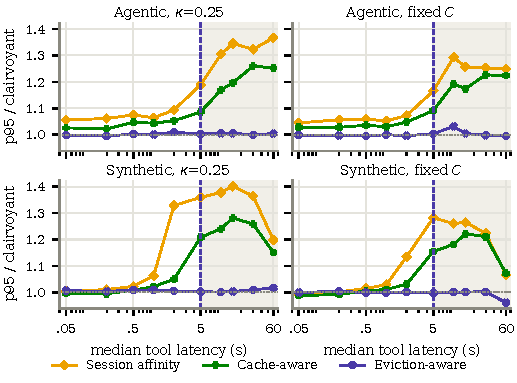
\includegraphics[width=\columnwidth]{figs/fig2_col.pdf}
\caption{p95 TTFT relative to the clairvoyant reference versus median tool latency at tight capacity ($\kappa=0.25$) and fixed absolute capacity $C$ ($N=4$, 70\% load, 5 seeds; shaded: beyond 5~s). Dashed: crossover.}
\label{fig:cross}
\end{figure}

\textbf{The tool-latency crossover (RQ3).} The \emph{crossover} is the smallest swept $\tau$ from which eviction-aware's lead over the best eviction-oblivious locality policy (per seed, the lower p95 of cache-aware and session affinity) is $\ge$5\% with its paired interval excluding zero, at that $\tau$ and every larger one (Fig.~\ref{fig:cross}, Table~\ref{tab:ext}). Up to 1--2~s eviction-aware leads the better locality policy by at most 4\%. \emph{Agentic:} for $\kappa\le1$ the crossover is at 5~s (7.5$\pm$3.9\% at $\kappa=0.25$, 6~ms; interval 3.6--11.4\%), the lead is established above 5\% from 10~s and plateaus at about 20\% (54--56~ms) at 30--60~s. With ample memory ($\kappa=2$) stickiness matches eviction awareness up to 5~s, but the crossover appears at 10~s, as $\rho$ falls from 33 to 2.9 over the sweep~\eqref{eq:rho}. \emph{Synthetic:} at $\kappa=0.25$ the crossover is at 5~s (16.8$\pm$3.7\%, 38~ms); the lead peaks at 15~s (21\%, 79~ms) and shrinks at 60~s, where $\rho<1$ and every locality policy misses alike. At $\kappa\ge1$ the 60~s lead is not significant, so the rule finds no crossover although the lead is $\ge$5\% and significant from 5~s ($\kappa=1$) or 10~s ($\kappa=2$) through 30~s. \emph{Scarce headroom:} halving $H$ moves the crossover to 500~ms (agentic) and 1~s (synthetic), as~\eqref{eq:rho} predicts. \emph{Fixed capacity:} with $C$ fixed, $\rho$ falls from 34 to 1.7 (agentic) and 22 to 1.0 (synthetic), and the crossover is again at 5~s on both workloads (7.7$\pm$2.9\%, 6~ms; 13.3$\pm$6.2\%, 24~ms); a memory budget that holds the idle sessions of 1~s tools needs the guard from about 5~s. At 5~s and fixed $C$ the lead is 6.6--7.2\% (agentic) and 10--23\% (synthetic) for $N\in\{2,8\}$. \textbf{Effect size versus model error.} With the cached-token term the lead at 5~s is 8\% (agentic) and 18\% (synthetic), no smaller, so this bias makes relative gaps conservative. The replay's absolute p95 error ($-$15 to $-$23\%) is about 12--19~ms at the 80~ms agentic p95 at 5~s, larger than the 6~ms agentic lead there, which therefore rests on the error being common to all policies; the synthetic leads (24--81~ms) and the agentic leads from 15~s on (26--56~ms at p95 of 150--230~ms) are as large as or larger than the error.

\begin{table}[t]
\centering\scriptsize
\caption{Eviction-aware lead over the best eviction-oblivious locality policy, \% (mean $\pm$ 95\% CI, 5 paired seeds) and ms in parentheses}
\label{tab:ext}
\setlength{\tabcolsep}{2pt}\renewcommand{\arraystretch}{0.9}
\resizebox{\columnwidth}{!}{\begin{tabular}{@{}rcccccc@{}}
\toprule
& \multicolumn{3}{c}{Agentic} & \multicolumn{3}{c}{Synthetic}\\
\cmidrule(lr){2-4}\cmidrule(l){5-7}
$\tau$ (s) & $\kappa=0.25$ & $\kappa=2$ & fixed $C$ & $\kappa=0.25$ & $\kappa=2$ & fixed $C$\\
\midrule
5 & 7.5$\pm$3.9 (6) & 4.0$\pm$2.3 (3) & 7.7$\pm$2.9 (6) & 16.8$\pm$3.7 (38) & 3.5$\pm$2.9 (3) & 13.3$\pm$6.2 (24)\\
10 & 13.8$\pm$2.8 (21) & 6.1$\pm$2.6 (5) & 13.4$\pm$3.2 (19) & 19.0$\pm$4.1 (62) & 9.0$\pm$4.9 (13) & 15.2$\pm$2.6 (41)\\
15 & 15.8$\pm$3.0 (32) & 9.4$\pm$3.9 (11) & 14.4$\pm$1.1 (26) & 21.1$\pm$5.9 (79) & 10.7$\pm$3.7 (20) & 18.0$\pm$1.3 (57)\\
30 & 20.6$\pm$1.6 (54) & 12.2$\pm$2.7 (22) & 18.6$\pm$1.9 (46) & 19.6$\pm$4.0 (81) & 10.0$\pm$1.7 (25) & 16.9$\pm$3.6 (62)\\
60 & 19.6$\pm$4.3 (56) & 16.4$\pm$2.3 (41) & 18.6$\pm$2.8 (51) & 11.7$\pm$2.4 (51) & 3.3$\pm$5.3 (8) & 9.1$\pm$8.8 (33)\\
\bottomrule
\end{tabular}}
\end{table}
\begin{table}[t]
\centering\scriptsize
\caption{Miss-cost decomposition at $\kappa=0.25$, 5~s median tool latency (means over 5 seeds)}
\label{tab:miss}
\setlength{\tabcolsep}{3pt}\renewcommand{\arraystretch}{0.92}
\begin{tabular}{@{}lrrrrrrr@{}}
\toprule
& hit & exp. & recomp./ & delay & hit p95 & tail & p95\\
Policy & \% & miss \% & miss & (ms) & (ms) & exp.\ \% & (ms)\\
\midrule
\multicolumn{8}{@{}l}{\emph{Agentic}}\\
Least-loaded & 76 & 4.5 & 447 & 12 & 66 & 63 & 203\\
Session affinity & 91 & 0.5 & 755 & 19 & 61 & 10 & 90\\
Cache-aware & 91 & 0.5 & 559 & 8 & 57 & 9 & 82\\
Eviction-aware & 91 & 0.4 & 619 & 6 & 53 & 9 & 76\\
Clairvoyant & 91 & 0.5 & 626 & 6 & 52 & 9 & 75\\
\midrule
\multicolumn{8}{@{}l}{\emph{Synthetic}}\\
Least-loaded & 63 & 15.4 & 752 & 18 & 113 & 81 & 339\\
Session affinity & 82 & 6.0 & 829 & 17 & 88 & 67 & 251\\
Cache-aware & 84 & 5.1 & 826 & 14 & 75 & 70 & 223\\
Eviction-aware & 83 & 5.2 & 768 & 6 & 53 & 90 & 185\\
Clairvoyant & 83 & 5.3 & 767 & 6 & 53 & 92 & 185\\
\bottomrule
\end{tabular}
\tabnote{exp.\ miss: requests recomputing $>$1024 previously computed prefix tokens; recomp./miss: recomputed tokens per miss; delay: TTFT minus the request's own isolated prefill time; tail exp.: share of the p95 tail that are expensive misses.}
\end{table}

\textbf{Mechanism: misses are not cheaper, they delay less.} At $\kappa=0.25$ and 5~s (Table~\ref{tab:miss}), eviction-aware and cache-aware reach the same hit rate and a similar share of expensive misses, and eviction-aware does \emph{not} make misses cheaper (+60$\pm$43 recomputed tokens per miss on agentic, $-$58$\pm$9 on synthetic traffic). It changes \emph{who waits for a miss}: the share of tail TTFT spent behind other requests is 7\% for eviction-aware against 23\% for cache-aware and 51\% for session affinity on agentic traffic (synthetic: 4\%, 32\%, 36\%). Affinity-based policies send a returning session needing a long recompute to its old replica, stalling the requests behind it; the TTFT-aware router places it where the backlog is shortest. \textbf{What is causal.} All policies in a cell see identical arrivals, so differences are policy effects; the decomposition rules out hit rate and miss cost, leaving queueing. Ablating the router's two ingredients ($\kappa\in\{0.25,1\}$, $\tau\in\{1,5,30\}$~s): TTFT placement with an eviction-blind index matches the full router on agentic traffic at 1--5~s ($-$0.8 to +2.1\%, intervals including zero) but is 14--20\% slower at 30~s, and 34\% slower on synthetic traffic already at 5~s; the eviction-aware index with longest-match placement is no better than cache-aware at 5~s (9.1\% vs.\ 8.2\% slower than the full router) and closes only half the gap at 30~s; without any queue term the cluster becomes unstable (p95 $>$50~s). Queue-aware placement is thus necessary and suffices under moderate shortage, and eviction awareness helps under severe shortage, only combined with it. Holding $\rho$ fixed, the agentic lead still grows with $\tau$ (7.0\% at 5~s to 15.0\% at 60~s, $\rho=3.5$) while the synthetic one shrinks (17.8\% to 6.1\%, $\rho=1.5$), so $\rho$ explains how the crossover moves with $\kappa$ and $H$ but is not a sufficient statistic. \textbf{Reconciling with SMetric.} SMetric finds session stickiness overloading instances at cluster scale (load imbalance 2.17$\times$ for session-ID routing)~\cite{r8}, whereas we find it near-optimal at normal headroom: at 5~s, session affinity's p95 grows from 67~ms at $\kappa=2$ to 90~ms at $\kappa=0.25$ and 143~ms with halved headroom, where eviction-aware routing is 36\% lower. SMetric's setting (32 instances, heavy session skew, reuse intervals up to about 100~s) lies in that pressured regime; this is a consistent reading, not a replication.

\begin{table}[t]
\centering\scriptsize
\caption{End-to-end latency (ms) and ITL (ms/token) for the principal policies ($N=4$, $\kappa=1$, 70\% load, means over 5 seeds)}
\label{tab:thpt}
\setlength{\tabcolsep}{2.5pt}\renewcommand{\arraystretch}{0.9}
\begin{tabular}{@{}lrrrrrrrrr@{}}
\toprule
& \multicolumn{3}{c}{Chat} & \multicolumn{3}{c}{Agentic} & \multicolumn{3}{c}{Synthetic}\\
\cmidrule(lr){2-4}\cmidrule(lr){5-7}\cmidrule(l){8-10}
Policy & E2E & p95 & ITL & E2E & p95 & ITL & E2E & p95 & ITL\\
\midrule
Least-loaded & 2935 & 7565 & 16.0 & 1302 & 3575 & 11.3 & 1236 & 2732 & 11.3\\
Session aff. & 3244 & 8273 & 17.6 & 1259 & 3468 & 11.1 & 1173 & 2604 & 10.9\\
Cache-aware & 2964 & 7756 & 16.1 & 1229 & 3373 & 10.9 & 1162 & 2574 & 10.8\\
Eviction-aware & 2856 & 7427 & 15.9 & 1237 & 3398 & 11.0 & 1194 & 2659 & 11.1\\
Clairvoyant & 2853 & 7363 & 15.8 & 1236 & 3390 & 11.0 & 1188 & 2642 & 11.1\\
\bottomrule
\end{tabular}
\end{table}

\textbf{Throughput and end-to-end latency.} Request and output-token throughput agree across policies to within 0.1\% at 70\% and 85\% load (agentic 9.26~req/s, 1025 output and 13,300 input tokens/s at 70\%), as expected for open-loop arrivals below saturation, so the TTFT gains carry no throughput cost. They carry over to end-to-end latency (Table~\ref{tab:thpt}): on agentic traffic eviction-aware lowers mean E2E by 65$\pm$8~ms (5.0\%) relative to least-loaded, and on chat by 388$\pm$37~ms (12\%) relative to session affinity. At this default configuration cache-aware has a slightly lower mean E2E than eviction-aware on agentic (8$\pm$7~ms) and synthetic traffic (32$\pm$26~ms), a small cost where eviction awareness brings no TTFT benefit. At 85\% load the picture is unchanged. The cache is full under every policy (resident occupancy 98--100\%); the policies differ in what they keep, not how much. From $N=2$ to 16, least-loaded's agentic p95 grows from 114 to 206~ms while session affinity stays at 62~ms; disabling prefix caching raises least-loaded p95 TTFT by 3.9$\times$ (agentic) and 1.4$\times$ (chat).

% =============================================================================
\section{Guidance (RQ4)}
\label{sec:guidance}

(1) \emph{Route agentic sessions for locality}: session affinity is nearly as good as longest-prefix routing when the cache is large enough. (2) \emph{Do not transfer chat intuitions}: for single-turn chat, session affinity is among the worst choices. (3) \emph{Never hash only the leading tokens} of a shared template. (4) \emph{Guard stickiness against eviction when tools take seconds} (from about 5~s with memory near the working set, 0.5~s when headroom is scarce, 10~s with ample memory), by queue-aware TTFT-based placement with a bounded LRU shadow of each replica's cache, as in SMetric~\cite{r8}; an eviction-aware index alone does not help. (5) \emph{Size KV memory for the idle-session working set}: estimate $W(\tau)$ from request logs with~\eqref{eq:cap} and check which side of the shortage the deployment is on.

% =============================================================================
\section{Limitations}
\label{sec:limits}

The multi-replica cluster is simulated and calibrated on single-GPU measurements, so we use it only to compare policies, and differences below its p95 error (15--23\%) rest on the error being common to all policies. Tool latencies beyond 60~s and saturated load are not studied. The MIG slice may exaggerate KV-pressure effects relative to a full GPU; we use one model, one engine version and one agentic domain; the chat prefixes are synthesised; and the simulator's eviction and admission approximate the engine's.

% =============================================================================
\section{Conclusion}
\label{sec:concl}

Tool-call latency, through the idle-session working set it creates, decides whether KV capacity changes how agentic requests should be routed. With fast tools, session affinity is near-optimal (62 vs.\ 58~ms p95 for the clairvoyant reference). From about 5~s with capacity at or below the working set (normalised or fixed), 0.5--1~s with scarce headroom, or 10~s with ample memory, an eviction guard with TTFT-based placement leads by 5--23\% (6--81~ms) at no throughput cost, not by making misses cheaper but by placing each session's recompute where it delays others least.

\section*{Acknowledgment}
An AI assistant (Claude, Anthropic) was used for drafting; the authors reviewed all content and take full responsibility for it. The agentic workload descriptor contains only numeric per-turn token counts and timings, with no prompts or clinical content.

\begin{thebibliography}{99}

\bibitem{r1} W. Kwon, Z. Li, S. Zhuang, Y. Sheng, L. Zheng, C. H. Yu, J. E. Gonzalez, H. Zhang, and I. Stoica, ``Efficient memory management for large language model serving with PagedAttention,'' in \emph{Proceedings of the 29th ACM Symposium on Operating Systems Principles (SOSP)}, 2023. [Online]. Available: \url{https://arxiv.org/abs/2309.06180}

\bibitem{r2} L. Zheng, L. Yin, Z. Xie, C. Sun, J. Huang, C. H. Yu, S. Cao, C. Kozyrakis, I. Stoica, J. E. Gonzalez, C. Barrett, and Y. Sheng, ``SGLang: Efficient execution of structured language model programs,'' in \emph{Advances in Neural Information Processing Systems 37 (NeurIPS)}, 2024. [Online]. Available: \url{https://arxiv.org/abs/2312.07104}

\bibitem{r3} V. Srivatsa, Z. He, R. Abhyankar, D. Li, and Y. Zhang, ``Preble: Efficient distributed prompt scheduling for LLM serving,'' in \emph{International Conference on Learning Representations (ICLR)}, 2025. [Online]. Available: \url{https://arxiv.org/abs/2407.00023}

\bibitem{r4} SGLang Team, ``SGLang v0.4: Zero-overhead batch scheduler, cache-aware load balancer, faster structured outputs,'' LMSYS Org Blog, Dec.\ 2024. [Online]. Available: \url{https://www.lmsys.org/blog/2024-12-04-sglang-v0-4/}

\bibitem{r5} NVIDIA, ``NVIDIA Dynamo documentation: Router design,'' accessed 2026-11-10. [Online]. Available: \url{https://docs.nvidia.com/dynamo/knowledge-base/modular-components/router/router-design}

\bibitem{r6} M. Ayoub, D. Harnik, T. Smith, K. Swain, X. Wang, H. Yin, and K. Yan, ``KV-cache wins you can see: From prefix caching in vLLM to distributed scheduling with llm-d,'' llm-d Blog, Sep.\ 2025. [Online]. Available: \url{https://llm-d.ai/blog/kvcache-wins-you-can-see}

\bibitem{r7} vLLM Project, ``vLLM production stack,'' 2025, accessed 2026-09-25. [Online]. Available: \url{https://github.com/vllm-project/production-stack}

\bibitem{r8} J. Wang, K. Lin, K. Zhang, J. Han, X. Wei, S. Shen, C. Fang, W. Yu, R. Chen, and H. Chen, ``SMetric: Rethink LLM scheduling for serving agents with balanced session-centric scheduling,'' arXiv preprint arXiv:2607.08565, 2026. [Online]. Available: \url{https://arxiv.org/abs/2607.08565}

\bibitem{r9} Huang Cheng, ``CacheRoute: Planned prefix-affinity routing for large-scale LLM serving,'' arXiv preprint arXiv:2608.19677, 2026, author name as displayed on arXiv. [Online]. Available: \url{https://arxiv.org/abs/2608.19677}

\bibitem{r10} vLLM Project, ``Automatic prefix caching (design documentation),'' 2025, accessed 2026-09-25. [Online]. Available: \url{https://docs.vllm.ai/en/latest/design/prefix_caching.html}

\bibitem{r11} D. Karger, E. Lehman, T. Leighton, R. Panigrahy, M. Levine, and D. Lewin, ``Consistent hashing and random trees: Distributed caching protocols for relieving hot spots on the world wide web,'' in \emph{Proceedings of the 29th Annual ACM Symposium on Theory of Computing (STOC)}, 1997, pp.~654--663.

\bibitem{r15} B. Gao, Z. He, P. Sharma, Q. Kang, D. Jevdjic, J. Deng, X. Yang, Z. Yu, and P. Zuo, ``Cost-efficient large language model serving for multi-turn conversations with CachedAttention,'' in \emph{USENIX Annual Technical Conference (ATC)}, 2024, pp.~111--126. [Online]. Available: \url{https://arxiv.org/abs/2403.19708}

\bibitem{r16} R. Abhyankar, Z. He, V. Srivatsa, H. Zhang, and Y. Zhang, ``InferCept: Efficient intercept support for augmented large language model inference,'' in \emph{Proceedings of the 41st International Conference on Machine Learning (ICML)}, ser. Proceedings of Machine Learning Research, vol.~235, 2024, pp.~81--95. [Online]. Available: \url{https://proceedings.mlr.press/v235/abhyankar24a.html}

\bibitem{r19} H. Li, R. He, Q. Mang, Q. Zhang, H. Mao, X. Chen, H. Zhou, H. Zhang, A. Cheung, J. Gonzalez, and I. Stoica, ``Continuum: Efficient and robust multi-turn LLM agent scheduling with KV cache time-to-live,'' arXiv preprint arXiv:2511.02230, 2025. [Online]. Available: \url{https://arxiv.org/abs/2511.02230}

\bibitem{r20} S. Tiwari, T. Chugh, N. Rickert, S. Peter, R. Mahajan, and H. Shen, ``CacheWise: Understanding workloads and optimizing KVCache management for efficiently serving LLM coding agents,'' arXiv preprint arXiv:2606.16824, 2026. [Online]. Available: \url{https://arxiv.org/abs/2606.16824}

\bibitem{r21} J. Wang, S. Eicher, K. Hakhamaneshi, and R. Pei, ``Optimizing LLM serving efficiency: Moving beyond KV cache reuse to token-load awareness with Ray Serve LLM,'' Anyscale Blog, Aug.\ 2026. [Online]. Available: \url{https://www.anyscale.com/blog/llm-kv-token-aware-routing}

\bibitem{r22} Z. Hong \emph{et al.}, ``Scheduling mixed RL rollouts beyond prefix locality,'' arXiv preprint arXiv:2608.11152, 2026. [Online]. Available: \url{https://arxiv.org/abs/2608.11152}

\bibitem{r23} Qwen Team, A. Yang, B. Yang \emph{et al.}, ``Qwen2.5 technical report,'' arXiv preprint arXiv:2412.15115, 2024. [Online]. Available: \url{https://arxiv.org/abs/2412.15115}

\bibitem{r24} Microsoft Azure, ``Azure LLM inference dataset 2023,'' 2023, accessed 2026-09-25. [Online]. Available: \url{https://github.com/Azure/AzurePublicDataset/blob/master/AzureLLMInferenceDataset2023.md}

\bibitem{r25} P. Patel, E. Choukse, C. Zhang, A. Shah, \'I. Goiri, S. Maleki, and R. Bianchini, ``Splitwise: Efficient generative LLM inference using phase splitting,'' in \emph{Proceedings of the 51st ACM/IEEE International Symposium on Computer Architecture (ISCA)}, 2024, source of the Azure LLM Inference Trace 2023 (github.com/Azure/AzurePublicDataset). [Online]. Available: \url{https://arxiv.org/abs/2311.18677}

\bibitem{r26} I. Gim, S.-s. Lee, and L. Zhong, ``Asynchronous LLM function calling,'' arXiv preprint arXiv:2412.07017, 2024. [Online]. Available: \url{https://arxiv.org/abs/2412.07017}

\bibitem{r27} B. Liu, H. Qiu, \'I. Goiri, R. Fonseca, R. Bianchini, and E. Choukse, ``Agentic coding in the wild: Characterizing GitHub Copilot at production scale,'' arXiv preprint arXiv:2608.00101, 2026. [Online]. Available: \url{https://arxiv.org/abs/2608.00101}

\bibitem{r28} C. Chang, Y. Zhou, K. Fu, D. An, T. Feng, H. Lu, S. Yao, P. Guo, Y. Yu, Y. Shan, B. Li, B. Yuan, and W. Wang, ``From LLM inference to agentic workloads: Characterization and implications for serving systems,'' arXiv preprint arXiv:2608.15127, 2026. [Online]. Available: \url{https://arxiv.org/abs/2608.15127}

\bibitem{r29} Y. Yuan, A. Nayak, S. Kundu, and N. Talati, ``Agentic AI workload characterization,'' arXiv preprint arXiv:2605.26297, 2026. [Online]. Available: \url{https://arxiv.org/abs/2605.26297}

\end{thebibliography}

\end{document}
